\subsection{Human Interface Design}
Users will engage with the system via a mobile application featuring an intuitive user interface (UI) that is accessible on Android devices, ensuring a seamless experience regardless of platform.
\subsubsection{Login and Registration Pages}
In order to use PedalPal, the User has to login first. If the user has not created an account yet, he/she can click on Sign Up to create a new accout. If the user has forgotten his/her password, he/she can reset it using the ”Forgot Password” button.
\begin{center}
\begin{tabular}{ccc}
    \includegraphics[scale=0.1]{ui-images/Register.png} & \includegraphics[scale=0.1]{ui-images/PhoneOTP.png} &    \includegraphics[scale=0.1]{ui-images/AccountSuccess.png}\\
    \textbf{Registration Page} & \textbf{Phone Authentication} & \textbf{Account Created}
\end{tabular}
\end{center}
\begin{center}
\begin{tabular}{ccc}
    \includegraphics[scale=0.1]{ui-images/Login.png} & \includegraphics[scale=0.1]{ui-images/EmailOTP.png} &\includegraphics[scale=0.1]{ui-images/ResetPassword.png}\\
    \textbf{Login Page} & \textbf{Email for Password Reset} & \textbf{Reset Password}
\end{tabular}
\end{center}

\subsubsection{Viewing Hubs and Booking a Ride}
The user sees a map which shows the location of the user along with the hubs present. They can either choose the hub on their map, or search it from the search box. Once a hub is selected, the details of the hub are displayed, including the number of available cycles. The user can choose to start a ride instantly, or book a cycle for a later time (available only for subscribed users). If the user wishes to book for later, they are presented with a time picker.
\begin{center}
\begin{tabular}{ccc}
    \includegraphics[scale=0.1]{ui-images/Dashboard.png} &
    \includegraphics[scale=0.1]{ui-images/HubSelection.png} &
    \includegraphics[scale=0.1]{ui-images/BookRideSubscribed.png}\\
    \textbf{Dashboard} & \textbf{Hub Selection} & \textbf{Book/Start Ride}
\end{tabular}
\end{center}

\subsubsection{Starting a Ride}
If the user wishes to ride instantly, they are presented with a QR code which they can scan to unlock the cycle. During the ride, statistics like ride time and current cost are shown to the user. Once the ride is over, the user can end the ride and the app will show the user the fare for the ride, and ask for feedback. The user can also report any issues with the cycle during the ride.
\begin{center}
\begin{tabular}{ccc}
    \includegraphics[scale=0.1]{ui-images/QR.png} & \includegraphics[scale=0.1]{ui-images/ActiveRide.png} & \includegraphics[scale=0.1]{ui-images/RideOver.png}\\
    \textbf{QR Code Scanner} & \textbf{Active Ride and Payment} & \textbf{Ride Over}
\end{tabular}
\end{center}

\subsubsection{User Feedback}
User has the option to give feedback on their riding experience and choose from various possible issues encountered during their ride and furnish a description thereof.
\begin{center}
\begin{tabular}{ccc}
    \includegraphics[scale=0.1]{ui-images/CycleIssues.png} & \includegraphics[scale=0.1]{ui-images/IssueDescription.png} & \includegraphics[scale=0.1]{ui-images/FeedbackSubmission.png}\\
    \textbf{Cycle Issues} & \textbf{Issue Description} & \textbf{Feedback Submitted}
\end{tabular}
\end{center}

\subsubsection{Subscription Model}
The option of booking rides in advance is only available for subscribed users. This option is greyed out in case the user is not subscribed. If the user taps on any greyed out option, an advertisement for subscribing is shown.
\begin{center}
    \begin{tabular}{cc}
        \includegraphics[scale=0.1]{ui-images/BookRideUnsubscribed.png} & \includegraphics[scale=0.1]{ui-images/Advertisement.png}\\
        \textbf{Booking Ride is Disabled} & \textbf{Advertisement}\\
        \textbf{for Unsubscribed Users} & 
    \end{tabular}
\end{center}

\subsubsection{Navigation Bar and Settings}
The navigation bar offers users a selection of choices, including accessing their wallet details, viewing ride history, adjusting settings, managing bookings, and logging out. Within the settings section, users can modify personal information and also have the option to subscribe for additional features.
\begin{center}
\begin{tabular}{cc}
    \includegraphics[scale=0.1]{ui-images/Navbar.png} & \includegraphics[scale=0.1]{ui-images/Settings.png}\\
    \textbf{Navigation Bar} & \textbf{Settings}
\end{tabular}
\end{center}

\subsubsection{Analytics and Wallet}
In the bookings page, users have access to both current and previous bookings, enabling them to track their activity. The history page provides users with a comprehensive overview of their ride history, detailing each ride's specifics. On the wallet page, users can monitor their balance and conveniently add funds to their wallet as needed.
\begin{center}
\begin{tabular}{ccc}
\includegraphics[scale=0.1]{ui-images/Bookings.png} & \includegraphics[scale=0.1]{ui-images/History.png} & \includegraphics[scale=0.1]{ui-images/Wallet.png}\\
\textbf{Bookings} & \textbf{History} & \textbf{Wallet}
\end{tabular}
\end{center}

\subsubsection{Admin Interface}
The admin interface serves as a control hub for managing both hubs and cycles. Admins possess the capability to introduce new hubs, inspect hub specifics, and regulate cycle operations. Furthermore, admins have access to comprehensive statistics, including total revenue metrics. They can also monitor user feedback and address reported issues effectively.

\begin{center}
\begin{tabular}{cc}
    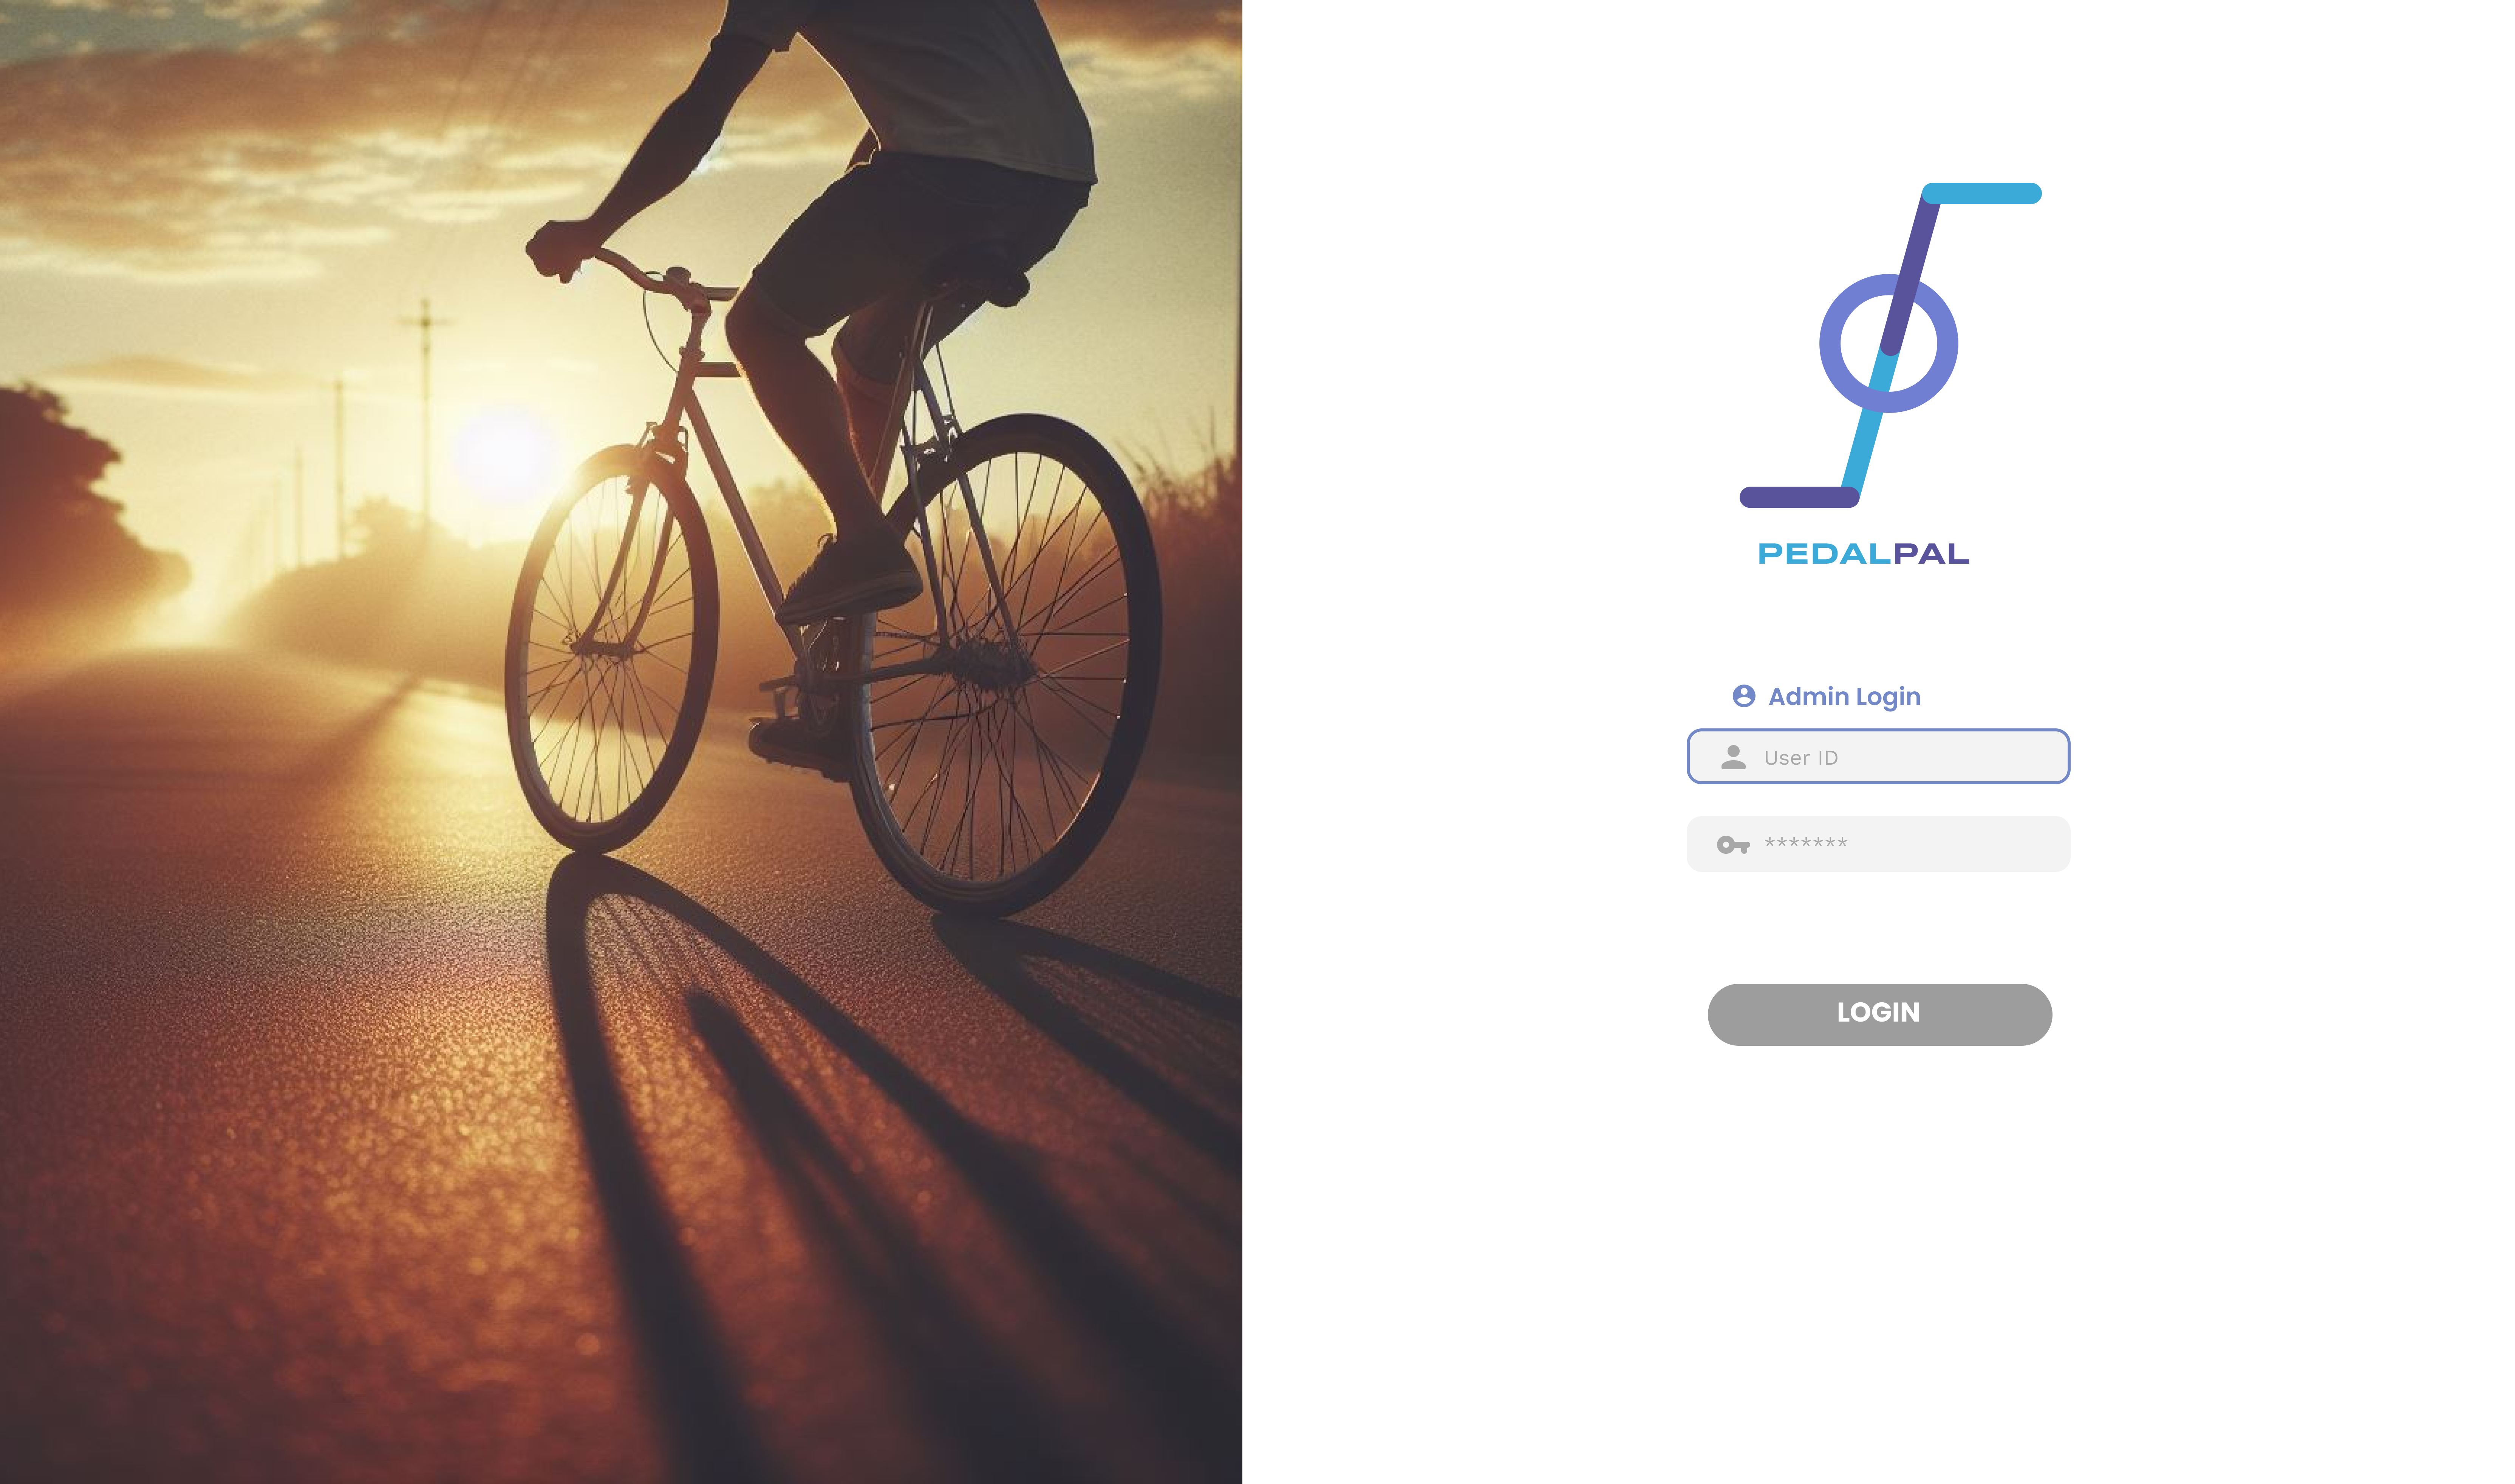
\includegraphics[scale=0.08]{ui-images/AdminLogin.png}\\
    \textbf{Admin Login}\\\\
    \includegraphics[scale=0.08]{ui-images/AdminDashboard.png}\\
    \textbf{Admin Dashboard}
\end{tabular}
\end{center}

